\documentclass[answers]{exam}
\usepackage[utf8]{inputenc}

\usepackage[dvipsnames]{xcolor}
\usepackage{amsmath}
\usepackage{amsfonts}
\usepackage{amsthm}
\usepackage{microtype}
\usepackage{siunitx}
\DeclareSIUnit\year{yr}
\usepackage{pgfplots}
\usepackage{graphicx}
\usepackage{sidecap}
\sidecaptionvpos{figure}{c}
\usepackage{float}
\usepackage{gensymb}
\usepackage{tkz-euclide}
\usetkzobj{all}
\usepackage{commath}
\usepackage{hyperref}
\usepackage{enumitem}
\usepackage{wasysym}

\renewcommand*{\thefootnote}{\fnsymbol{footnote}}

\newtheorem*{thm}{Theorem}
\newtheorem*{iden}{Identity}
\newtheorem*{lemma}{Lemma}
\theoremstyle{definition}
\newtheorem*{defn}{Definition}
\newtheorem*{ex}{Example}

% russian integral
\usepackage{scalerel}
\DeclareMathOperator*{\rint}{\scalerel*{\rotatebox{17}{$\!\int\!$}}{\int}}

% \qformat{Question \thequestion: \thequestiontitle\hfill}

\begin{document}

\section*{NCEA Level 3 Physics (Modern Physics)}
When an electric current is passed through a low-pressure gas, light is given out;
this phenomenon is used in (for example) neon lights. The light given out is of
interest to us because it is only emitted in a few specific frequencies, dependent
on the gas.

\begin{center}
  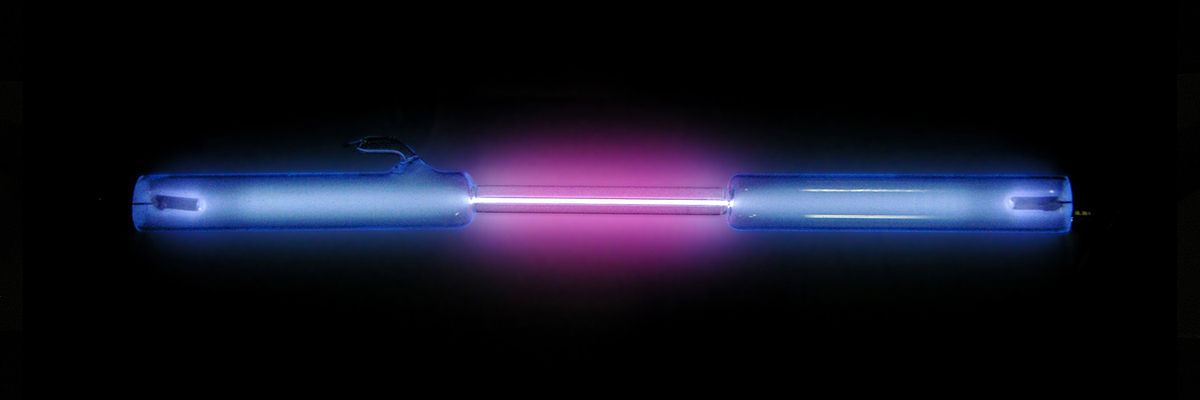
\includegraphics[width=\textwidth]{hydrogen-light}
\end{center}
If a high voltage is passed through low-pressure hydrogen, the tube glows with a pale
violet light; we can then pass this light through a diffraction grating to split out
its component frequencies. This produces the emission spectra shown here (the first showing the
locations of the visible spectra, the second the locations of the five series (clusters)).
\begin{center}
  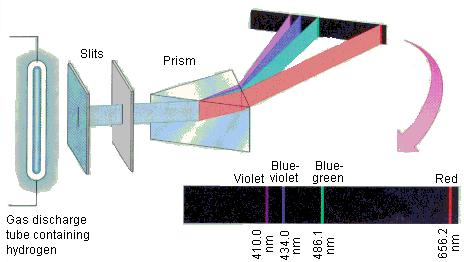
\includegraphics[width=0.6\textwidth]{hydrogen1}

  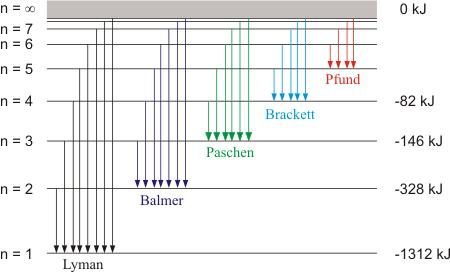
\includegraphics[width=0.6\textwidth]{hydrogen2}
\end{center}

It is possible to describe the series of wavelengths in the visible spectrum using
a formula constructed by J~J~Balmer in 1885:
\begin{displaymath}
  \frac{1}{\lambda} = R\left( \frac{1}{2^2} - \frac{1}{L^2} \right)
\end{displaymath}
where $ L $ is the number of each emission line starting from 3, and $ R \approx \SI{1.097e7}{\per\metre} $.

The formula can be extended to deal with the other invisible spectra:
\begin{displaymath}
  \frac{1}{\lambda} = R\left( \frac{1}{S^2} - \frac{1}{L^2} \right)
\end{displaymath}
Here, $ S $ is the \textit{series number}. For visible light, the series number is $ S = 2 $,
and this denotes the so-called \textit{Balmer series}. The value of $ L $ starts at $ S + 1 $ for
each series.

\begin{center}
\begin{tabular}{|c|c|c|c|}\hline
  \textbf{Series name} & \textbf{Location} & $ S $ & $ L $\\\hline
  Lyman & UV & 1 & 2, 3, ...\\
  Balmer & Visible & 2 & 3, 4, ...\\
  Paschen & IR & 3 & 4, 5, ...\\
  Brackett & IR & 4 & 5, 6, ...\\
  Pfund & IR & 5 & 6, 7, ...\\\hline
\end{tabular}
\end{center}

This behaviour is intimately related to the behaviour of electrons in the atom. In order to
explain it, we must delve deeper into the structure of the atom.

In 1911, Ernest Rutherford (of Nelson) postulated a model of the atom consisting of a small
positive nucleus containing most of the mass of the atom surrounded by tiny orbiting electrons.
However, this model was soon found to have several problems:
\begin{itemize}
  \item The orbiting electrons must be accelerating, but no additional energy is being provided ---
        so they should be radiating energy and should eventually fall into the nucleus.
  \item It doesn't explain why only some energies are emitted when the atom is excited.
\end{itemize}

Niels Bohr proposed a revised model of the atom in 1913. He postulated that electrons could
only remain in stable orbits with certain fixed energies, known as \textit{energy levels},
and that electrons move from one orbital to another by either emitting or absorbing a particular
amount of energy fom light.

Suppose a photon of wavelength $ \lambda $ is emitted by an electron moving from one energy level
to another in a hydrogen atom. We can use the formula above to perform some calculations.
Since $ f = \frac{c}{\lambda} $, we have that $ f = cR \left( \frac{1}{S^2} - \frac{1}{L^2} \right) $
and so $ E = hf = hcR \left( \frac{1}{S^2} - \frac{1}{L^2} \right) $ and
\begin{displaymath}
  E = \frac{hcR}{S^2} - \frac{hcR}{L^2}.
\end{displaymath}
In other words, the energy of the emitted photon is the difference between two electron energy levels.

This also implies that electrons in a hydrogen atom only exist at energy levels given by
\begin{displaymath}
  E = -\frac{hcR}{n^2}
\end{displaymath}
for $ n \in \mathbb{N} $.
The energy levels are negative, since electrons are bound to the nucleus. If $ E \geq 0 $,
then electrons can leave the nucleus. As $ n \to\infty $, $ E \to 0 $. Hence as we move the
electrons away from the nucleus, their binding energy decreases.

The second spectra diagram above shows a diagram of the energy levels, and shows that we
can explain the emission spectrum of the hydrogen atom using the Bohr model of the atom. When
an electron drops from a higher energy level to a lower energy level, a photon of light
is released; and as light is absorbed by an electron, it climbs to a higher energy level.

The wavelength of emitted (or absorbed) light is given by
\begin{displaymath}
  \frac{1}{\lambda} = R\left( \frac{1}{S^2} - \frac{1}{L^2} \right)
\end{displaymath}
where $ L $ is the higher energy level and $ S $ is the lower level.

\subsection*{Questions}
Useful data: $ c \approx \SI{2.99e8}{\metre\per\second} $, $ h \approx \SI{6.63e-34}{\joule\second} $,
$ e \approx \SI{1.6e-19}{\coulomb} $, $ \SI{1}{\electronvolt} \approx \SI{1.6e-19}{\joule} $, $ R \approx \SI{1.097e7}{\per\metre} $

\begin{questions}
  \question Calculate the wavelength and frequency of the first line in the Balmer series.
  \question Calculate the wavelength and frequency of the second line in the Pfund series.
  \question Calculate the limiting (shortest possible) wavelength at the end of the Paschen series.
  \question Find the energy value of the lowest electron energy level in a hydrogen atom.
  \question An electron falls from the third to the second energy level in a hydrogen atom. Calculate:
    \begin{parts}
      \part The loss of energy of the electron
      \part The energy of the emitted photon
      \part The frequency of the emitted photon
    \end{parts}
  \question
    \begin{parts}
      \part If the frequency of the photon emitted by an electron of a particular jump is \SI{6.91e14}{\hertz},
            find the energy of the photon.
      \part Determine the wavelength of the photon.
    \end{parts}
  \question In the hydrogen atom, when an electron drops from energy level 4 (\SI{-1.36e-19}{\joule}) to
            energy level 2 (\SI{-5.44e-19}{\joule}), a photon with wavelength $ \lambda = \SI{4.88e-9}{\metre} $ is emitted.
    \begin{parts}
      \part Calculate the energy of the photon.
      \part Calculate the frequency of the photon.
      \part Calculate the value of Planck's constant.
    \end{parts}
\end{questions}

\end{document}
